\chapter{Aplicaciones existentes}
\label{cap:aplicacionesexistentes}
\todo{Echa un vistazo por aquí. He dividido las aplicaciones buscadas en sus características y he añadido al final unas conclusiones}

En este apartado se describen aplicaciones existentes que permiten al profesorado la gestión del proceso de calificación de su alumnado junto con un análisis comparativo de los mismos.

\section{EducamosCLM}

Esta aplicación web de la Junta de Comunidades de Castilla-La Mancha\cite{educamosclm} es la aplicación de gestión de alumnado por excelencia en los centros educativos públicos. 

Busca dotar de herramientas de gestión y comunicación para el profesorado, el alumnado y los padres mediante un entorno seguro, flexible e intuitivo. Además también posee un módulo para realizar trámites en los centros.

\begin{figure}[h]
\centering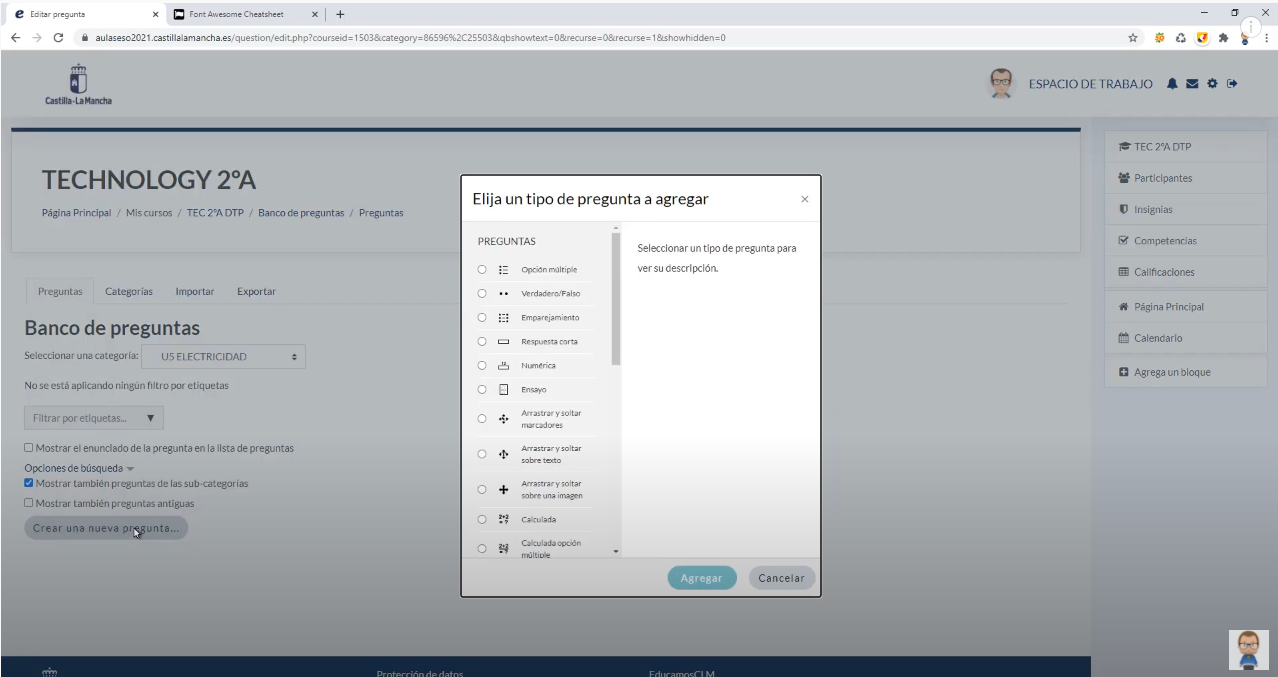
\includegraphics[width=1\linewidth]{figs/educamosCLM2.png}
\caption{Crear un examen en EducamosCLM.\cite{educamosclmyoutube}}
\label{Fig:educamosCLM}
\end{figure}

A continuación se muestran las características principales de EducamosCLM comparadas con las de esta aplicación. Cabe mencionar que, la primera y la que se ha considerado más notoria, es que EducamosCLM es exclusiva para los colegios públicos de Castilla-La Mancha, mientras que la desarrollada es libre y se podría usar en cualquier colegio sin restricciones regionales, público o privado.

\textbf {Seguimiento del curso.}
    En este apartado, los maestros pueden publicar las notas de sus alumnos para que estos y los padres las vean en cualquier momento, así como las faltas de asistencia y la trayectoria escolar que lleva el alumno durante el curso.
    En la vista de los alumnos, estos podrán subir sus trabajos on-line, que le aparecerán al maestro para que pueda descargarlos e introducir la calificación en el sistema. Este sistema también permite a los alumnos pedir tutorías con los maestros.


\section{Google Classroom}

Google Classroom es una aplicación para navegador web y para smartphone\cite{googleclassroom} desarrollada por Google que permite la comunicación entre maestros y alumnos, así como la gestión y organización de trabajos mediante Google Drive.

\begin{figure}[h]
\centering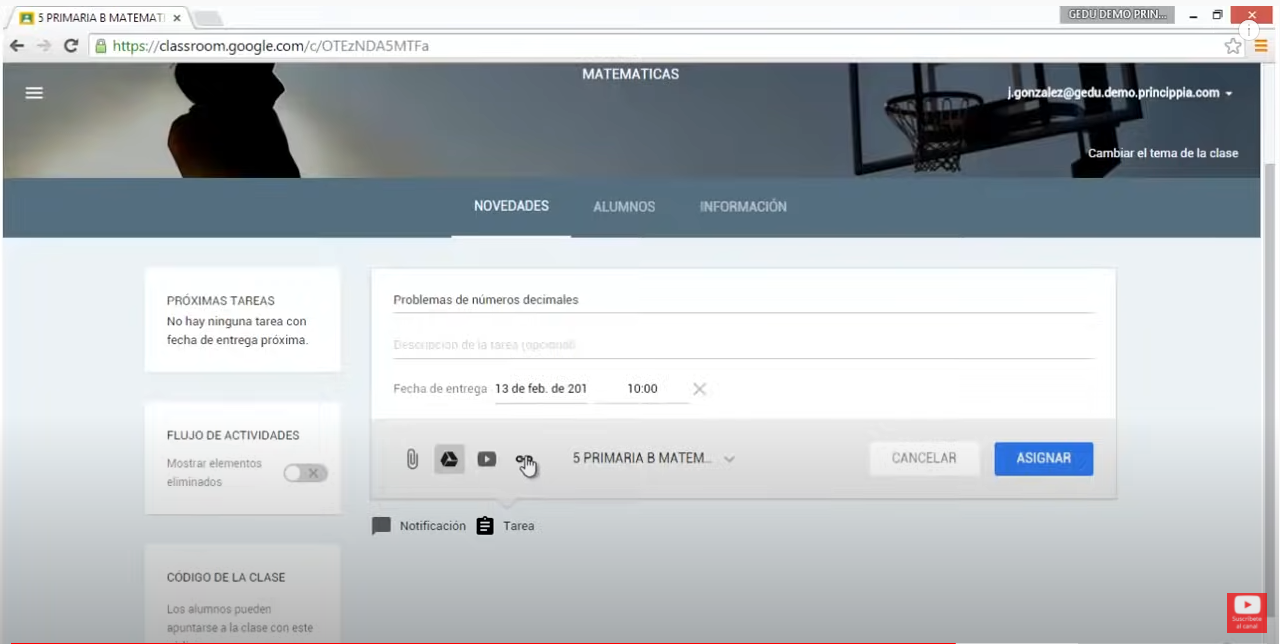
\includegraphics[width=1\linewidth]{figs/googleclassroom.png}
\caption{Crear una tarea en Google Classroom.\cite{googleclassroomyoutube}}
\label{Fig:googleclassroom}
\end{figure}

A continuación se muestran las características principales de Google Classroom comparadas con las de esta aplicación.

\textbf {Orientado a maestros y alumnos.} Principalmente, Google Classroom está pensado tanto para maestros como para alumnos, por lo que es muy completo. Tiene herramientas para programar entregas, reuniones y para que el maestro pueda comunicarse mediante mensajes de texto con un alumno o con toda la clase.

\textbf {Archivos en la nube.} Todos los archivos que se suben van directamente a Google Drive. De esta forma se almacenan todos en el mismo sitio, pero de forma ordenada, y cada alumno y docente puede acceder a estos archivos mediante una cuenta Google aceptada en el curso. 

\textbf {Personalizable mediante aplicaciones externas.} Google Classroom es una aplicación flexible: permite la integración de aplicaciones como Classcraft, Pear Deck o Quizizz, posibilitando una completa personalización de la experiencia tanto para los alumnos como para los maestros. Debido a la generalización de la herramienta, es muy versátil y se puede usar para cualquier curso, tanto de primaria como de secundaria.
	

\section{Additio}
\label{sec:additio}

Additio es una aplicación para navegador web y smartphone\cite{additio} que permite gestionar las notas del alumnado y las competencias que tiene cada metodología, planificar las clases y la comunicación con padres y alumnos.

\begin{figure}[h]
\centering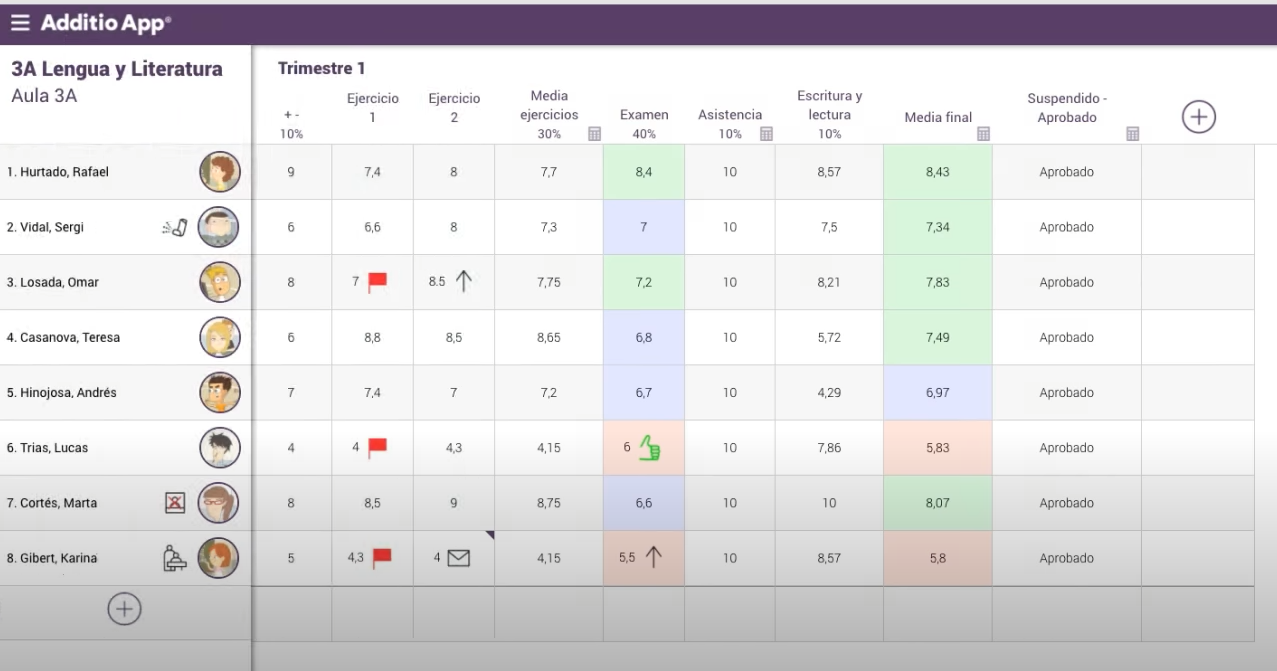
\includegraphics[width=1\linewidth]{figs/additio.png}
\caption{Gestión de notas en Additio.\cite{additioyoutube}}
\label{Fig:additio}
\end{figure}

A continuación se muestran las características principales de Additio comparadas con las de la aplicación desarrollada en este documento.

Additio está diseñada tanto para maestros como para Centros y permite, como las anteriores, gestionar notas y trabajos, la asistencia a clase y la comunicación entre padres, maestros y alumnos. Sin embargo, tiene una característica nueva que no se había encontrado en las aplicaciones descritas anteriormente: la posible introducción de competencias para las pruebas.

\textbf {Aplicación on-line multiplataforma.} Additio puede usarse en smartphone, tablet u ordenador, lo que permite un mayor seguimiento de las actividades, independiente de la localización del docente.
 
\textbf {Calendario y agenda.} Additio también contiene un calendario y una agenda para establecer citas con alumnos y padres.

\textbf {Pocas opciones de personalización de interfaz.} Additio no permite modificar la interfaz o los colores a gusto del usuario.


\section{Análisis y conclusiones}

\textbf{Carmen, esto ¿no debería estar quizá en las conclusiones del documento, donde me dijiste que pusiera la tabla comparando las aplicaciones? siento que tenemos conclusiones en dos partes diferentes.}

Para concluir este capítulo, se realiza un pequeño análisis de la diferencia entre las aplicaciones elegidas.

En general, se puede ver que el punto en el que más se diferencia la aplicación desarrollada con las que se han investigado es la dificultad de uso. Si bien es cierto que las aplicaciones mencionadas poseen más funcionalidades y son más flexibles, debido a esto tienen un grado de dificultad mucho mayor que la aplicación desarrollada.

A continuación se listan más diferencias:
\begin{itemize}
\item \textbf{Personalización de la interfaz.} Ninguna de las aplicaciones investigadas posee un grado de personalización tan grande como la desarrollada. Aunque a primera vista podría parecer de poca importancia, la realidad es que si la aplicación presenta dificultades para ser leída con facilidad, la usabilidad no es la misma y el usuario se siente menos cercano a la aplicación.
\item \textbf{Sin conexión a Internet.} Todas las aplicaciones investigadas tienen conexión a Internet, y aunque el hecho de no tenerla a priori pueda parecer un paso atrás en el desarrollo de una aplicación, la realidad es otra. La decisión de desarrollar una aplicación de escritorio sin conexión a Internet tiene varias ventajas, entre ellas el acceso en cualquier lugar, aunque no se posea Internet; una mayor seguridad de los datos debido a la imposibilidad de fugas de datos personales y el centrado del foco de atención del docente en su trabajo, ya que no tendrá que salir de la aplicación para realizar ningún otro trámite.
\item \textbf{Aplicación de escritorio.} Unida con las razones anteriores, las aplicaciones de escritorio son más personalizables, y si bien pueden requerir de actualizaciones manuales, esto permite que se puedan realizar a la vez para todos los usuarios del mismo Centro de tal forma que todos los docentes tengan siempre la misma versión de la aplicación.
\end{itemize}

Como conclusión final, se considera que las aplicaciones investigadas poseen una curva de aprendizaje mucho mayor que la aplicación desarrollada y un nivel pobre de personalización a gusto del usuario.